\documentclass[handout,x11names]{beamer}
\usepackage{etex,beamerfoils}
\usepackage{array,pifont,amsmath,latexsym,epsfig,amsfonts,yfonts}
\usepackage{amstext,amsopn,amsxtra,amsgen,amsbsy,amscd,amssymb,dcolumn,graphicx,setspace,pgfplots,booktabs,natbib}
\usepackage[normalem]{ulem}
\usepackage[all]{xy}
\beamertemplatetheoremsnumbered
\setbeamertemplate{caption}[numbered]
\usetheme{Copenhagen}
\definecolor{NewBlue}{RGB}{4, 114, 155}
\definecolor{magenta}{cmyk}{0,1,0,0}
\usecolortheme[named=NewBlue]{structure}
%\usecolortheme[named=SkyBlue4]{structure}

\newcommand{\D}{\displaystyle}
\newcommand{\E}{\begin{eqnarray*}}
\newcommand{\F}{\end{eqnarray*}}
\newcommand{\EE}{\begin{eqnarray}}
\newcommand{\FF}{\end{eqnarray}}
\newcommand{\IZ}{\begin{itemize}}
\newcommand{\ZI}{\end{itemize}}
\newcommand{\EN}{\begin{enumerate}}
\newcommand{\NE}{\end{enumerate}}
\newcommand{\itemc}{\item[$\circ$]}
\newcommand{\IZdash}{\begin{itemize} \renewcommand{\labelitemi}{-}}
\newcommand{\tn}{\textnormal}

% New commands to assist Beamer
\newcommand{\itemi}{\item<1->}
\newcommand{\itemii}{\item<2->}
\newcommand{\itemiii}{\item<3->}
\newcommand{\itemiv}{\item<4->}
\newcommand{\itemv}{\item<5->}
\newcommand{\itemvi}{\item<6->}
\newcommand{\itemvii}{\item<7->}
\newcommand{\itemviii}{\item<8->}
\newcommand{\itemix}{\item<9->}
\newcommand{\itemx}{\item<10->}

\newcommand{\itemci}{\item[$\circ$]<1->}
\newcommand{\itemcii}{\item[$\circ$]<2->}
\newcommand{\itemciii}{\item[$\circ$]<3->}
\newcommand{\itemciv}{\item[$\circ$]<4->}
\newcommand{\itemcv}{\item[$\circ$]<5->}
\newcommand{\itemcvi}{\item[$\circ$]<6->}
\newcommand{\itemcvii}{\item[$\circ$]<7->}
\newcommand{\itemcviii}{\item[$\circ$]<8->}
\newcommand{\itemcix}{\item[$\circ$]<9->}
\newcommand{\itemcx}{\item[$\circ$]<10->}


\newcommand{\fr}{\frame}
\newcommand{\ft}{\frametitle}
\newcommand{\ons}{\onslide}
\newcommand{\tc}{\textcolor}

\pgfplotsset{height =7cm,compat=1.7,width=7cm,
    standard/.style={
    	unit vector ratio*=1 1 1,
        axis x line=middle,
        axis y line=middle,
        enlarge x limits=0.15,
        enlarge y limits=0.15,
        every axis x label/.style={at={(current axis.right of origin)},anchor=north west},
        every axis y label/.style={at={(current axis.above origin)},anchor=north east}
    }
}
\newcommand{\drawge}{-- (rel axis cs:1,0) -- (rel axis cs:1,1) -- (rel axis cs:0,1) \closedcycle}
\newcommand{\drawle}{-- (rel axis cs:1,1) -- (rel axis cs:1,0) -- (rel axis cs:0,0) \closedcycle}

\usetikzlibrary{patterns}
\usetikzlibrary{arrows}
\usetikzlibrary{shapes}

\renewcommand{\bibsection}{}

% Watermark example: https://texblog.org/2012/02/17/watermarks-draft-review-approved-confidential/
\usepackage{draftwatermark}
\SetWatermarkText{This content is protected and may not be shared uploaded or distributed.}
\SetWatermarkScale{0.25}
\SetWatermarkAngle{0}
\SetWatermarkColor[gray]{1.0}
\setbeamercolor{background canvas}{bg=}%transparent canvas

\title[Prescott's RBC Model\hspace{2em}\insertframenumber/
\inserttotalframenumber]{Prescott's RBC Model}
\author{Brian C.~Jenkins \\ ~ \\University of California, Irvine}

\begin{document}

\frame{\maketitle}

\fr{
\ft{Introduction}

\IZ
\item Finn Kydland and Edward Prescott were awarded the 2004 Nobel Memorial Prize in Economics, in part, for their contribution to our understanding of the driving forces behind business cycles.

\

\item They pioneered a new approach to studying business cycles that became known as \emph{real business cycle} or  \emph{RBC} theory.


%\

%\item RBC theory was novel in that it emphasized optimizing behavior -- utility and profit maximization -- 
%
%\item \cite{Prescott1986}
%
%\cite{KydlandPrescott1982}, \cite{KydlandPrescott1988}
\ZI
}

\fr{
\ft{Introduction}
\IZ
\defcitealias{Prescott1986}{Edward Prescott's 1986 article}
\item \citetalias{Prescott1986} ``Theory Ahead of Business Cycle Measurement'' provides an overview of models he developed with Kydland.

\

\item The model described on pages 11-17 -- which I'll call \emph{Prescott's model} -- explains the endogenous co-movement of output, employment, consumption, and investment over the business cycle.

\ZI
}

\fr{
\ft{Introduction}

\IZ
\itemi Prescott's model is \emph{decentralized}: \pause the household makes some decisions and profit-maximizing firms make others and allocations are settled in markets with prices.

\

\itemiii Below, I describe a \emph{centralized} version of Prescott's model: \pause the representative household owns all resources and makes all allocation decisions

\

\itemv The only consequence of the difference is that Prescott is able to model the equilibrium prices of labor and capital.
\ZI
}

\fr{
\ft{Centralized RBC Model with Labor}

\IZ
\item A \emph{representative household} lives for an infinite number of periods.

\


\itemii Each period: consumes $C_t$ and allocates share of available time $L_t$ to labor activities.

\

\itemiii Flow of utility in period $t$:

\EE
\log (C_t) + \varphi \log (1-L_t),
\FF
where $1-L_t$ is the share of the household's time spent enjoying leisure.


	

\ZI

}


\fr{
\ft{Centralized RBC Model with Labor}

\IZ

\itemi The \emph{expected present value of lifetime utility} to the household from consuming $C_0, C_1, C_2, \ldots $ is denoted by $U_0$:
	\EE
	U_0 & = & \log (C_0)  + \varphi \log(1-L_0)  \nonumber \\
	    &  & \; \; \; \; \; \; \; +\,  \beta \big[E_0 \log (C_1) + \varphi \log (1-L_1)\big] \nonumber\\
	    &  & \; \; \; \; \; \; \; +\,  \beta^2 \big[E_0 \log (C_2) + \varphi \log (1-L_2)\big] \nonumber\\
	    &  & \; \; \; \; \; \; \; +\,  \cdots \\
	\pause & = & E_0\sum_{t = 0}^{\infty} \beta^t \big[\log (C_t) + \varphi \log (1-L_t)\big],  \label{eqn:infinite_per_det_utility}
	\FF
	

\ZI

}

\fr{
\ft{Centralized RBC Model with Labor}

\IZ
\item The household enters period 0 with capital $K_0>0$.

\

\itemii Production in period $t$:
	\EE
	F(A_t,K_t,L_t) & = & A_t K_t^{\alpha}L_t^{1-\alpha}
	\FF
where TFP $A_t$ is stochastic:
	\EE
	\log A_{t+1} & = & \rho \log A_t + \epsilon_{t+1}
	\FF
	
\itemiii The household's resource constraint is:
    \EE
    C_t + K_{t+1} & = & A_t K_{t}^{\alpha}L_t^{1-\alpha}  + (1-\delta)K_t,
    \FF
 for $t = 0, 1, 2, 3,\ldots$

\ZI

}


\fr{
\ft{Centralized RBC Model with Labor}

\IZ
\item \textbf{Optimization problem}: Each period the household chooses:

	\EN
	\item Consumption for the current period
	\item Labor the current period
	\item Capital for the subsequent period
	\NE

	to maximize its expected present value of lifetime utility.
	
\

\item We'll solve the problem for period 0 and then generalize the solution to apply to all periods $0, 1, 2, \ldots$

\ZI
}


\fr{
\ft{Centralized RBC Model with Labor}

\IZ
\item In period 0, the household solves:
	\EE
	&&\max_{C_0,L_0,K_1} \; E_0\sum_{t=0}^{\infty}\beta^t\big[\log (C_t) + \varphi \log (1-L_t) ]\\\nonumber\\
	&& \; \; \; \;  \; \; \; \; \tn{s.t.} \; \; \; \; C_t + K_{t+1} = A_t K_{t}^{\alpha}L_t^{1-\alpha}  + (1-\delta)K_t\nonumber
	\FF 

\
	
\itemii The problem can be written as a choice of $L_0$ and $K_1$ only:
	\EE
	&&\max_{L_0,K_1} \; E_0\sum_{t=0}^{\infty}\beta^t\big[\log ( A_t K_{t}^{\alpha}L_t^{1-\alpha}  + (1-\delta)K_t - K_{t+1}) \nonumber\\
	&& \; \; \; \; \; \; \; \; \; \; \; \; \; \; \; \; \; \; \; \; \; \; \; \; \; \; \; + \, \varphi \log(1-L_t) \big]
	\FF 

\ZI

}


\fr{
\ft{Centralized RBC Model with Labor}

\IZ
\item The first-order condition with respect to $L_0$ is:
	\EE
	\frac{(1-\alpha) A_0 K_0^{\alpha}L_0^{-\alpha}}{C_0} & = & \frac{\varphi}{1-L_0}
	\FF
	
\

\itemii The first-order condition with respect to $K_1$ is:
	\EE
	\frac{1}{C_0} & = & \beta E_0 \left[\frac{\alpha A_{1} K_{1}^{\alpha-1}L_{1}^{1-\alpha} + 1 - \delta}{C_1}\right]
	\FF
\ZI
}


\fr{
\ft{Centralized RBC Model with Labor}

\IZ

\item The household solves the same problem in periods $1, 2, 3, \ldots$

\

\itemii So given $K_0>0$ and $A_0$, the equilibrium paths for labor, consumption, capital, and TFP are described described by:
	\EE
	\pause \frac{\varphi}{1-L_t} & = & \frac{(1-\alpha)A_tK_t^{\alpha}L_t^{-\alpha}}{C_t} \\
	\pause \frac{1}{C_t} & = & \beta E_t \left[\frac{\alpha A_{t+1}K_{t+1}^{\alpha - 1}L_{t+1}^{1-\alpha} + 1 - \delta}{C_{t+1}}\right]\\
	\pause C_t + K_{t+1} & = & A_{t} K_t^{\alpha}L_t^{1-\alpha} + (1-\delta) K_t\\
	\pause \log A_{t+1} & = & \rho \log A_t + \epsilon_{t+1}
	\FF


\ZI
}


\fr{
\ft{Centralized RBC Model without Labor}

\IZ

\item Computing numeric values for consumption and capital is not trivial. Recall the Euler equation:
	\EE
	\frac{1}{C_t} & = & \beta E_t \left[\frac{\alpha A_{t+1}K_{t+1}^{\alpha - 1}L_{t+1}^{1-\alpha} + 1 - \delta}{C_{t+1}}\right]
	\FF
	
\

\item Consumption at date $t$ depends on the \emph{expectation} of consumption at date $t+1$ which in turn depends on the expectation of consumption at date $t+2$ and so on.


\

\item Solving the problem requires numerical methods like those employed in the \texttt{linearsolve} Python package.

\ZI
}


\fr{
\begin{figure}[h] \caption{\label{fig_014_intro_prescott_rbc_gdp_irs} \textbf{Kydland and Prescott RBC model with labor.} Impulse responses to a one percent shock to TFP in period 5.}
\begin{center}\hspace*{-.5cm}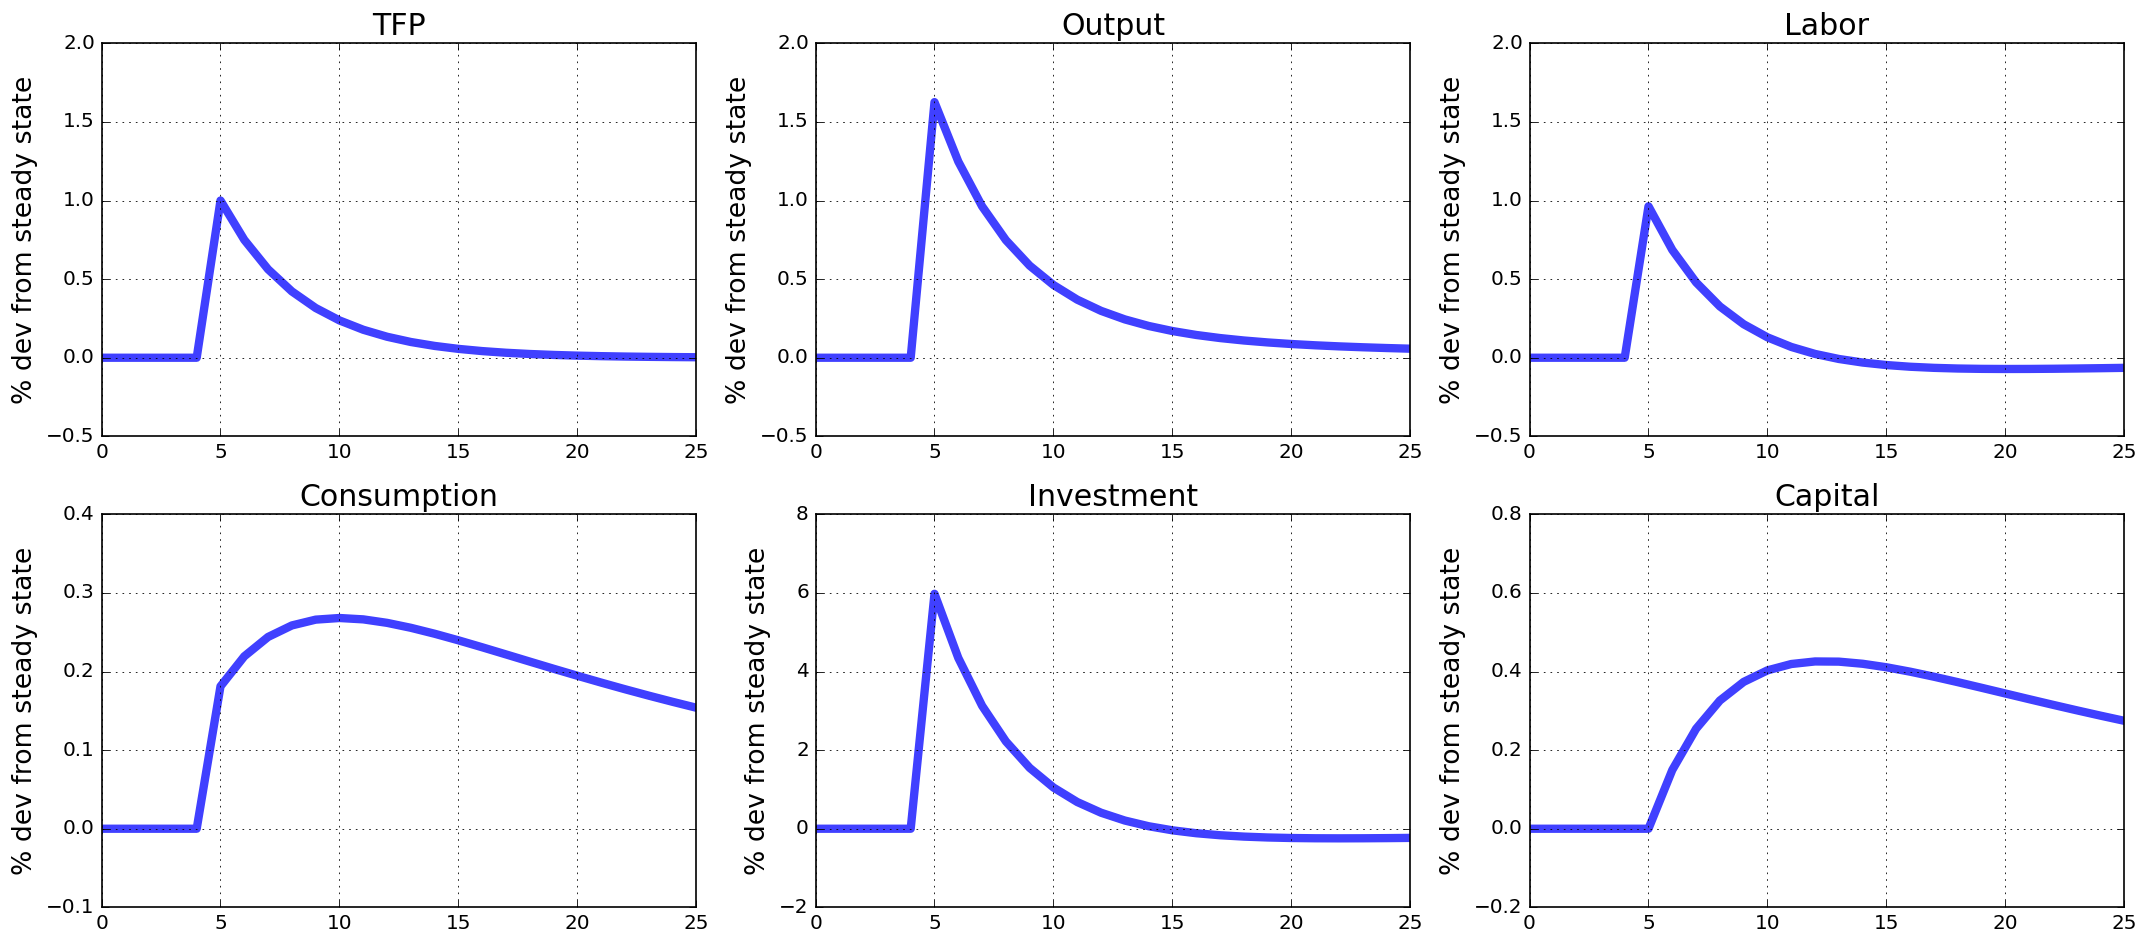
\includegraphics[height = 4.5cm]{fig_014_intro_prescott_rbc_gdp_irs.png}\end{center}
\end{figure}
}


\fr{
\begin{figure}[h] \caption{\label{fig_014_intro_prescott_rbc_gdp} \textbf{GDP.} Actual and simulated data from Prescott's RBC model for the US from April 1948 to April 2022. {\tiny Source: FRED}.}
\begin{center}\hspace*{-.5cm}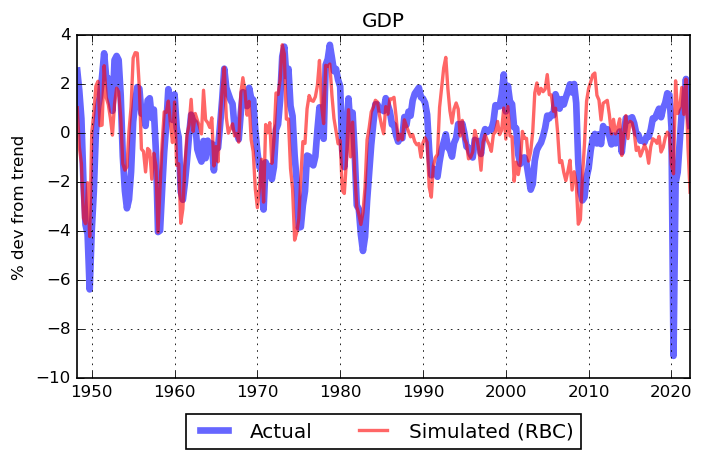
\includegraphics[height = 4.5cm]{fig_014_intro_prescott_rbc_gdp.png}\end{center}
\end{figure}
}

\fr{
\begin{figure}[h] \caption{\label{fig_014_intro_prescott_rbc_consumption} \textbf{Consumption.} Actual and simulated data from Prescott's RBC model for the US from April 1948 to April 2022. {\tiny Source: FRED}.}
\begin{center}\hspace*{-.5cm}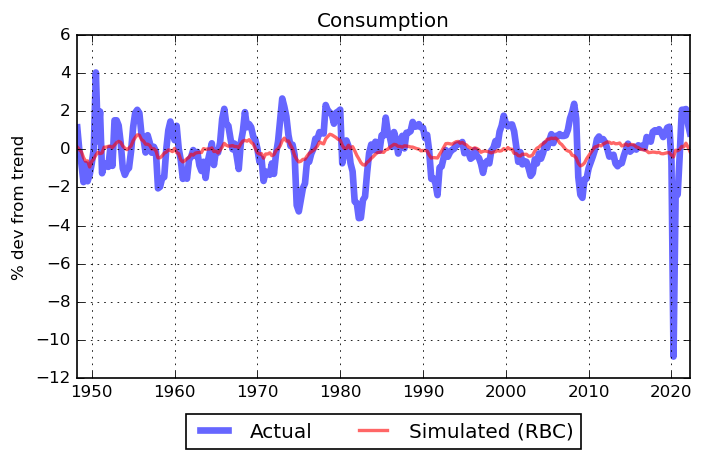
\includegraphics[height = 4.5cm]{fig_014_intro_prescott_rbc_consumption.png}\end{center}
\end{figure}
}

\fr{
\input{figure_014_intro_prescott_rbc_investment.tex}
}

\fr{
\input{figure_014_intro_prescott_rbc_labor.tex}
}


\fr{
\begin{table}[h] \caption{\label{tab014_intro_prescott_rbc_stds} \textbf{Standard deviations.} Actual data and data simulated from RBC models with and without labor. Units are percent deviations from trend. {\tiny Source: FRED}.}
\begin{center}\hspace*{-.5cm}

\begin{tabular}{lccc}
\toprule
{} &  Actual & RBC (w/o labor) &  RBC (w/ labor) \\
\midrule
Output      &    1.69 &            0.94 &            1.53 \\
Consumption &    1.34 &            0.22 &            0.33 \\
Investment  &    7.41 &            3.39 &            5.60 \\
Labor       &    2.06 &             $-$ &            0.91 \\
\bottomrule
\end{tabular}
\end{center}
\end{table}
}


\fr{
\begin{table}[h] \caption{\label{tab014_intro_prescott_rbc_corrs} \textbf{Correlations with GDP.} Actual data and simulated data. {\tiny Source: FRED}.}
\begin{center}\hspace*{-.5cm}

\begin{tabular}{lccc}
\toprule
{} &  Actual & RBC (w/o labor) &  RBC (w/ labor) \\
\midrule
Consumption &    0.81 &            0.61 &            0.59 \\
Investment  &    0.84 &            0.99 &            0.99 \\
Labor       &    0.88 &             $-$ &            0.98 \\
\bottomrule
\end{tabular}
\end{center}
\end{table}
}

\fr{
\ft{Centralized RBC Model without Labor}

\IZ
\item Summary analysis of the Prescott RBC Model with labor:

	\IZ
	\itemii Substantial improvement in explaining output, consumption, investment, and labor volatility
	\itemiii Still under-predicts consumption-GDP correlation and over-predicts investment-GDP correlation
	\ZI
	
	\
	
\item Criticisms

	\EN
	\itemiv Attributes \emph{all} business cycle fluctuations to TFP shocks
	\itemv Attributes \emph{all} labor fluctuations to \emph{voluntary} changes in labor supply.
	\NE

\ZI
}


\fr{
\ft{References}
\bibliographystyle{aer}
\bibliography{comp_econ_references.bib}
}

\end{document}